\vspace{-2pt}
\section{Experiment Setup}
\label{sec:exp}
\vspace{-2pt}
\subsection{Environments and Tasks}
\label{sec:envs}
% We evaluate LLM agents in three symbolic environments designed to study learning from scratch and independent of task-specific engineering. All environments are minimal, fully controllable, and stripped of real-world priors to support clean analysis. Specifically, \textbf{Bandit} tests risk-sensitive symbolic reasoning under stochastic feedback; \textbf{Sokoban} requires irreversible multi-step planning in a deterministic setting; and \textbf{Frozen Lake} combines planning with probabilistic transitions. Visualizations and environment illustrations are deferred to Appendix~\ref{app:env-setting}. We also include experiments on more realistic task, WebShop~\cite{yao2022webshop} and include the results in Appendix~\ref{app:webshop}.

We evaluate LLM agents on four environments spanning symbolic and realistic decision-making: \textbf{Bandit} tests risk-sensitive reasoning under noisy feedback; \textbf{Sokoban} requires irreversible symbolic planning; \textbf{Frozen Lake} combines planning with probabilistic transitions; and \textbf{WebShop} involves natural language grounding and web environment interaction. 
The first three symbolic environments are deliberately minimal and fully controllable to support clean analysis, while WebShop introduces realistic task structure and language input. Environment visualizations are in Appendix~\ref{app:env-setting}.
\vspace{-5pt}

\subsection{Training Settings}
In our main experiments, we train Qwen-2.5 Instruct 0.5B models for three symbolic tasks and its 3B variant for the challenging WebShop. We also report various model performance in Appendix~\ref{app:largermodelabaltion}. Models are trained with StarPO variants on H100 GPUs for 100-200 rollout–update iterations. Each batch samples $P{=}8$ prompts, with $N{=}16$ rollouts per prompt, up to 5 turns and 10 actions. Policy updates use GRPO or PPO with GAE ($\gamma{=}1.0, \lambda{=}1.0$), Adam optimizer, entropy bonus ($\beta{=}0.001$), and a response-format penalty ($-0.1$). More details can be found in Appendix~\ref{app:train-eval-setting}.
\vspace{-5pt}

\subsection{Evaluation Metrics}
We evaluate on 256 fixed prompts per environment with temperature $T{=}0.5$, truncating episodes after 5 turns. Metrics include: 
\textbf{(i)} success rate (task completion),
\textbf{(ii)} rollout entropy (exploration),
\textbf{(iii)} in-group reward variability (behavioral diversity),
\textbf{(iv)} response length (reasoning verbosity),
and \textbf{(v)} gradient norm (training stability).
All are computed over validation instances. More details can be found in Appendix~\ref{app:metric-setting}.
\vspace{-5pt}


% \subsection{Environments and Tasks}
% \label{sec:envs}
% We evaluate LLM agents in three \textbf{minimal yet comprehensive} symbolic environments designed to isolate core decision-making challenges. These environments are minimal, controllable, and stripped of real-world priors, enabling clean analysis of reasoning emergence and learning dynamics. Specifically, \textbf{Bandit} (Figure~\ref{fig:bandit-intro}) tests risk-sensitive symbolic reasoning under stochastic feedback; \textbf{Sokoban} (Figure~\ref{fig:sokoban_env_example}) requires irreversible multi-step planning in a deterministic setting; and \textbf{Frozen Lake} (Figure~\ref{fig:frozenlake_env_example}) combines planning with probabilistic transitions. More details can be found in Appendix~\ref{app:env-setting}.


% \begin{figure}[t]
%     \centering
%     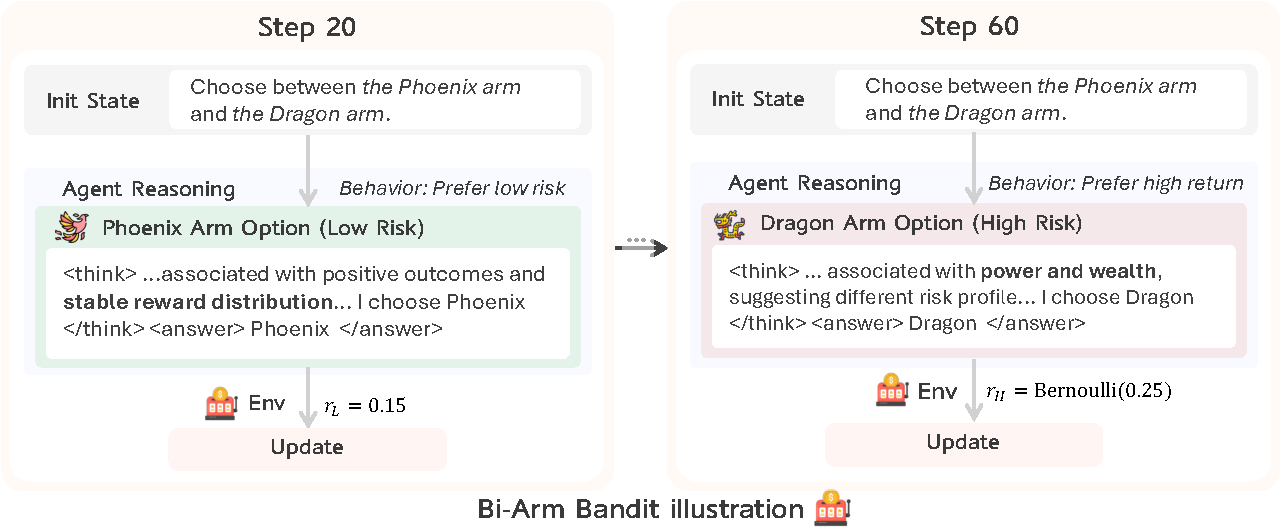
\includegraphics[width=\linewidth]{figures/example.pdf}
%     \caption{\textbf{Bi-Arm Bandits environment.} The agent chooses between a low-risk arm (Phoenix) and a high-risk yet high-reward arm (Dragon), each linked to symbolic semantics. The agent learns to choose stable reward at early stages and reasons to pursue maximal expected reward and shift toward strategic risk-taking. }
%     \label{fig:bandit-intro}
% \end{figure}



% \begin{figure}[t]
% \centering
% \begin{minipage}{0.48\textwidth}
% \centering
% 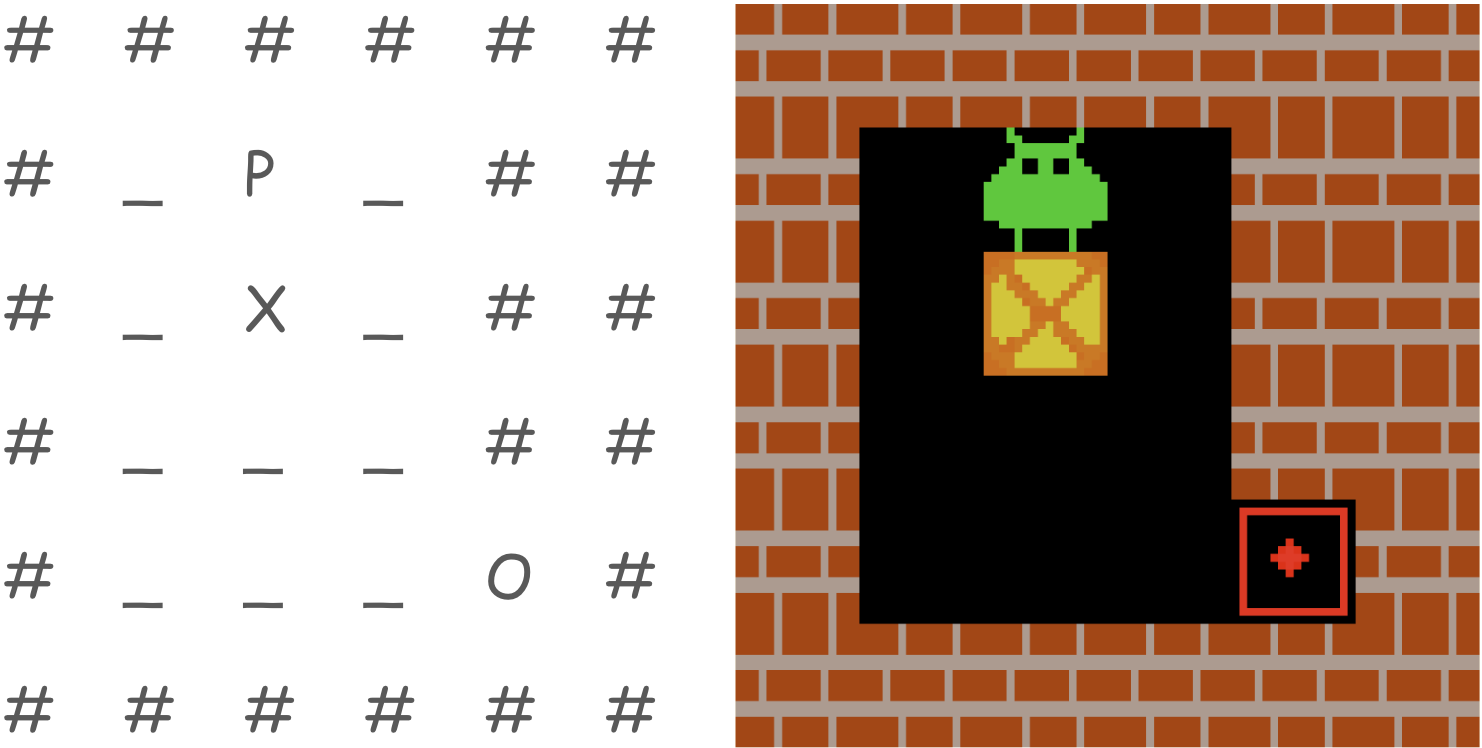
\includegraphics[width=0.8\linewidth]{figures/sokoban_env_example.png}
% \subcaption{Sokoban Environment. Actions are irreversible and the boxes cannot be pulled back which needs foresight and careful planning.}
% \label{fig:sokoban_env_example}
% \end{minipage}
% \hfill
% \begin{minipage}{0.48\textwidth}
% \centering
% 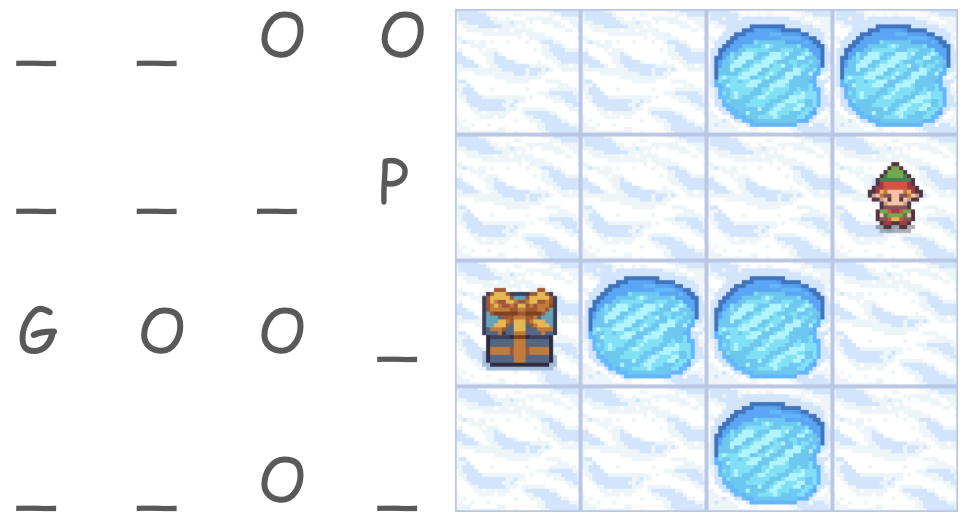
\includegraphics[width=0.8\linewidth]{figures/frozenlake_env_example.png}
% \subcaption{FrozenLake Environment. Each agent move may randomly slip to a side direction, requiring the agent to adapt under uncertainty.}
% \label{fig:frozenlake_env_example}
% \end{minipage}
% \caption{ \textbf{Sokoban and Frozen Lake environments.}
% For each environment, the left shows the agent-observed text rendering; the right is a visual illustration.
% (a) Sokoban is a deterministic multi-turn puzzle where the agent pushes boxes onto targets. (b) Frozen Lake combines multi-turn reasoning and stochasticity where the agent needs to reach the gift to succeed.
% }
% \label{fig:combined_environments}
% \end{figure}







% \input{tables/sokoban_main}
% \input{tables/frozen_lake}


% \subsection{Settings}
% Our primary experiments utilize the instruction-tuned 0.5B Qwen-2.5 model~\citep{qwen2.5}. 
% Unless otherwise noted, we implement the reward normalization strategy with prompt size $P$ as $8$, rollout size $K$ as $16$, update batch size $E$ as $32$, and maximum rollout loops $L$ capped at $200$.
% For comprehensive experimental parameters, please refer to Appendix~\ref{app:exp-setting}.

% For dataset generation, Bi-Arm Bandits use a consistent prompt with fixed reward distribution, while the training/evaluation set of Sokoban/Frozen Lake are synthesized automatically.

% \subsection{Bi-Arm Bandits}
% We develop Bi-Arm Bandits (Figure~\ref{fig:bandit-intro}) as the simplest environment to evaluate RAGEN's reasoning behavior in \textbf{stochastic environments} as an agent. It presents two arms with names of rich semantic symbolism (e.g., Dragon vs Phoenix), evaluating evolution of model reasoning capabilities to forming and updating hypotheses during training.



% The environment consists of two options: a low-risk arm (lo-arm) delivering consistent, fixed rewards and a high-risk arm (hi-arm) with higher expected value but greater variance. The hi-arm follows a Bernoulli distribution with probability p of yielding reward 1 and probability (1-p) of yielding 0. We establish the constraint $P(r_L > r_H) > 0.5$, where $r_L$ and $r_H$ represent the rewards from low-risk and high-risk arms respectively, ensuring the low-risk option outperforms the high-risk option in most individual trials despite the hi-arm's higher expected value. This design allows us to quantitatively assess cumulative reward optimization while qualitatively evaluating models' reasoning capabilities under uncertainty.



% \paragraph{Experiment Setup} For the hi-arm $H$ and lo-arm $L$, we set $L \sim \mathcal{N}(0.2, 0.1)$, $H \sim 0.75\times\mathcal{N}(0.1, 0.1) + 0.25 \times\mathcal{N}(1, 0.1)$. This setup ensures $P(L > H) > 0.5$ while maintaining meaningful variance in outcomes. We set name Dragon for hi-arm and Phoenix for lo-arm as default setting, and swap their names for a contrastive reverse setting. 
% During training, we set prompt size to 1, rollout size to 128, update batch size to 128, model update steps size to 200, and a kl-penalty of 0.001. The model is evaluated on its strategy to choose the hi-arms, which returns higher rewards in expectation.



% \paragraph{Results} We present results in Figure~\ref{fig:bandit-results}. We find RAGEN models learn to choose hi-arms faster than no-think-RL and maintains steady on their choices, showing the effectiveness and robustness of reasoning-reinforced agent training. We also find that evolving on default setting converges slower than evolving on reverse setting, showing that models may have strong initial beliefs about which symbol represents high-reward at first, which may influence reasoning towards action strategies or model training. We further analyze this in \S\ref{sec:ana-reason}.


% \subsection{Sokoban}
% We use Sokoban, a grid-based puzzle game implemented in OpenAI Gym\footnote{https://github.com/mpSchrader/gym-sokoban}, as our testing environment for \textbf{multi-turn} dynamics. The game state consists of an $N \times N$ grid where each cell is either a wall, empty space, player position, target position, or box. At each timestep, the agent selects one of four actions (\textit{up}, \textit{down}, \textit{left}, \textit{right}) to either move or push an adjacent box, aiming to push every box on a target. Reward mechanism consists of action penalty $-0.1$, every box on target $+1$, every box off target $-1$, and completion: $+10$.

% \paragraph{Experiment Setup} We set environment size to $6 \times 6$, box count to $1$, max turns to $5$, format penalty of $1$, KL-penalty of $0.001$. 

% \paragraph{Results} 

% We present results on the Sokoban task in Table~\ref{tab:sokoban_main}. From the results, we find RAGEN performs significantly better than no-think-RL, showing how RAGEN could handle multi-turn agent dynamics through reasoning.


% \subsection{Frozen Lake}
% We employ the grid-based puzzle Frozen Lake in OpenAI Gym\footnote{\url{https://gymnasium.farama.org/environments/toy_text/frozen_lake/}}, as our testing environment for \textbf{both stochastic and multi-turn} dynamics. It consists of an NxN grid containing start position, goal position, frozen tiles, and holes. The agent selects up/down/left/right at each step, but may slip with a probability $p$ where each action succeeds with probability $\frac{1}{3}$ and may result in perpendicular movement with probability $\frac{2}{3}$, introducing significant stochasticity to the environment.
% The reward is +1 for reaching the goal and 0 otherwise. Episodes terminate upon reaching the goal or falling into a hole.

% \paragraph{Experiment Setup} Most experiment settings are similar to Sokoban environment, while for Frozen Lake we set environment size 4x4.


% \paragraph{Results} We evaluate on metrics same as Sokoban.  Results are shown in Table~\ref{tab:frozen_main}. We find RAGEN outperforms no-think-RL even under such stochastic environments, showing how RAGEN could handle both multi-turn and stochastic dynamics.

% RAGEN adopts Inductive Grouping with Asymmetric Min-Clip Normalization, where the specific grouping criteria is detailed below.
% We compare three established baselines:
% \vspace{-8pt}
% \begin{itemize}
% \item Reasoning-Disabled StarPO: Ablates the reasoning component to analyze its impact
% \item State-level grouping: Uses conventional grouping methods without inductive properties
% \item No reward normalization: Uses raw reward signals to evaluate normalization benefits
% \end{itemize}
% \vspace{-8pt}


% Detailed configurations
% % , if not otherwise noted,
% can be found in Appendix~\ref{app:exp-setting}.
% % [TODO: Please paste base.yaml and ppo.yaml as is in papers in appendix].


% As shown in the Figure~\ref{fig:rico} (Right), each loop of RICO has a prompt size $P$ (each with different initial states $s_0$). The LLM generates $N$ trajectories each prompt, and is updated with an update batch size of $E$ and number of loops $L$. This leads to total gradient steps $S=\frac{L\cdot N\cdot P}{E}$.
% \paragraph{Experiment Setup} We set environment size to 6x6, box count to 1, max turns to 5, prompt size to 4, rollout size to 8, update size to 32, model update step size to 200, format penalty of 1, kl-penalty of 0.001[PINGYUE: Add appendix]. We compare our results with Supervised Fine-Tuning (SFT), no-think-RL as baselines. SFT datasets are observation-action trajectories from Breadth-First Search (BFS) without reasoning processes. For no-think-RL, we force the model to generate answers without thinking by removing any generated tokens not inside the <answer> tags. Other settings of no-think-RL are same as RICO.
% \begin{figure}[H]
%     \centering
%     \includegraphics[width=\linewidth]{figures/plot_task_performance.pdf}
%     \caption{Performance comparison with Baselines}
%     \label{fig:performance_sokoban}
% \end{figure}

% We evaluate on four metrics: valid or effective actions, success rate, and turns (or trajectory lengths in tokens) used to complete tasks. Valid actions are those in a correct answer format, and effective actions are those that changes the state (sometimes model may take meaningless moves towards a wall when they are beside it, which does not change state).
% Results are shown in Table~\ref{tab:sokoban_main}. From the results, we find RAGEN > no-think-RL > SFT, showing how RAGEN could handle multi-turn dynamics.
% We evaluate on two metrics: turns (or trajectory lengths in tokens) used to complete tasks and success rate. Results are shown in Table~\ref{tab:sokoban_main}. From the results, we find RAGEN > no-think-RL > SFT, showing how RAGEN could handle multi-turn dynamics.


% We find a consistent model evolve within three phases: initial low selection of both arms due to incorrect output format, followed by preferring lo-arm for stable baseline rewards, and finally shifting to hi-arm for higher expected returns.

% We pose several reasoning examples to support these claims. At step 10, trajectory 2, the model says "Phoenix signifies wealth and the prospect of prosperity, while Dragon implies danger and security.". At step X.... These examples show that language model can leverage reasoning to support its claims to consistently obtain high rewards when the reward functions is stochastic.


% \paragraph{Experiment Setup} Most experiment settings are similar to Sokoban environment, while for Frozen Lake we set environment size 4x4. We compare also our results with Supervised Fine-Tuning (SFT) and no-think-RL.

% \begin{figure}[H]
%     \centering
%     \includegraphics[width=\linewidth]{figures/plot_task_performance.pdf}
%     \caption{Performance comparison with Baselines}
%     \label{fig:performance_frozenlake}
% \end{figure}

% \paragraph{Results} We evaluate on the two metrics similar to Sokoban.  Results are shown in Table~\ref{tab:frozen_main}. From the results, we find RAGEN > no-think-RL > SFT even under such random environments, showing how RAGEN could handle both multi-turn and random dynamics.






